%\documentclass[12pt,a4paper]{article}

\setlength{\parindent}{0.1 in}
%\setlength{\parskip}{0.1 in}
\setlength{\oddsidemargin}{0.25 in}
\setlength{\evensidemargin}{-0.25 in}
\setlength{\topmargin}{-0.5 in}
\setlength{\textwidth}{7.0 in}
\setlength{\textheight}{9.5 in}
\setlength{\headsep}{0.45 in}

%\usepackage[fleqn]{amsmath}
%\usepackage{amsfonts,graphicx}
\usepackage{amsmath,amsfonts,graphicx}
\usepackage[fleqn]{mathtools}
\usepackage{setspace}
\usepackage[colorlinks=false, pdfborder={0 0 0}]{hyperref}
\usepackage[nottoc]{tocbibind}
\usepackage{tocloft}
\usepackage[outermargin=2 in]{geometry}
\usepackage{scrextend}
\usepackage{tensor}
\usepackage{cancel}
\usepackage{slashed}


%Adding `Appendix' to the appendices
\usepackage[toc,page]{appendix}

%Add a bullet point to description items
\usepackage{enumitem}

%Mathematics
\usepackage{braket}
\usepackage{ulem}
\usepackage{xcolor}
\usepackage[font={small,it}]{caption}

\bibliographystyle{unsrt}

% Packages that Gavin uses
\usepackage{url}
\usepackage[font=footnotesize]{caption}
\usepackage[font=footnotesize]{subcaption}
\usepackage[]{microtype}
\usepackage{balance}
\usepackage{cite}
\usepackage{lmodern}
\usepackage[T1]{fontenc}
\usepackage{doi}

% Nice typesetting of SI units
\usepackage{siunitx}
\sisetup{range-phrase=--}
\sisetup{separate-uncertainty = true}

% SImons packages
\usepackage{float}





%
%   This file is part of the APS files in the REVTeX 4.1 distribution.
%   Version 4.1r of REVTeX, August 2010
%
%   Copyright (c) 2009, 2010 The American Physical Society.
%
%   See the REVTeX 4 README file for restrictions and more information.
%
% TeX'ing this file requires that you have AMS-LaTeX 2.0 installed
% as well as the rest of the prerequisites for REVTeX 4.1
%
% See the REVTeX 4 README file
% It also requires running BibTeX. The commands are as follows:
%
%  1)  latex apssamp.tex
%  2)  bibtex apssamp
%  3)  latex apssamp.tex
%  4)  latex apssamp.tex
%
\documentclass[%
% reprint,
twocolumn,
%superscriptaddress,
%groupedaddress,
%unsortedaddress,
%runinaddress,
%frontmatterverbose, 
%preprint,
%showpacs,preprintnumbers,
%nofootinbib,
%nobibnotes,
%bibnotes,
 amsmath,amssymb,
 aps,
%prl,
%prb,
%rmp,
%prstab,
%prstper,
%floatfix,
]{revtex4-1}

\usepackage{graphicx}% Include figure files
\usepackage{dcolumn}% Align table columns on decimal point
\usepackage{bm}% bold math
\usepackage[colorlinks=false, pdfborder={0 0 0}]{hyperref}% add hypertext capabilities
%\usepackage[mathlines]{lineno}% Enable numbering of text and display math
%\linenumbers\relax % Commence numbering lines

%\usepackage[showframe,%Uncomment any one of the following lines to test 
%%scale=0.7, marginratio={1:1, 2:3}, ignoreall,% default settings
%%text={7in,10in},centering,
%%margin=1.5in,
%%total={6.5in,8.75in}, top=1.2in, left=0.9in, includefoot,
%%height=10in,a5paper,hmargin={3cm,0.8in},
%]{geometry}


%Mathematics
\usepackage{braket}
\usepackage[normalem]{ulem} % Not sure what this is for but definitely should keep normal italic \emph{}
\usepackage{xcolor}
%New commands
%Maths
\newcommand{\beq}{\begin{equation}}
\newcommand{\eeq}{\end{equation}}
\newcommand{\beqn}{\begin{equation*}}
\newcommand{\eeqn}{\end{equation*}}
\newcommand{\bea}{\begin{align}}
\newcommand{\eea}{\end{align}}
\newcommand{\p}{\partial}
\newcommand{\trace}[1]{\mathrm{Tr}\left[#1 \right]}
\newcommand{\ptrace}[2]{\mathrm{Tr}_{#1} \left[ #2 \right]}
\newcommand{\bpmat}{\begin{pmatrix}}
\newcommand{\epmat}{\end{pmatrix}}
\newcommand{\vv}[1]{\mathbf{#1}}
\newcommand{\mat}[1]{\uuline{#1}}
\newcommand{\norm}[1]{\| #1 \|}
\newcommand{\op}[1]{\mathbb{#1}}
\newcommand{\vhat}[1]{\hat{\vv{#1}}}

%Renewed commands, in order for them to take arguments with automatically adjusted brackets 
\renewcommand{\dim}[1]{\mathrm{dim}\left( #1\right)}
\renewcommand{\det}[1]{\mathrm{det} \left( #1 \right)}
\renewcommand{\exp}[1] {\mathrm{exp} \left[ #1 \right]}


%\mathbb Letters
\newcommand{\identity}{\mathbb{I}}
\newcommand{\inreal}{\mathbb{R}}
\newcommand{\incomplex}{\mathbb{C}}

%Redefine Braket
\renewcommand{\braket}[1]{\left\langle #1 \right\rangle}

%Integration
\newcommand{\intd} {\mathrm{d}}

%Operators
\newcommand{\phihat}{\hat{\phi}}
\newcommand{\xhat}{\hat{x}}
\newcommand{\phat}{\hat{p}}
\newcommand{\Dhat}{\hat{D}}
\newcommand{\Hhat}{\hat{H}}
\newcommand{\ahat}{\hat{a}}
\newcommand{\bhat}{\hat{b}}
\newcommand{\chat}{\hat{c}}
\newcommand{\Phihat}{\hat{\Phi}}

%Channels
\newcommand{\channel}[3]{\mathcal{#1}^{#2 \rightarrow #3}}


%Caligraphy letters
\newcommand{\cl}[1]{\mathcal{#1}}
\newcommand{\Hilbert}{\mathcal{H}}
\newcommand{\calN}{\mathcal{N}}
\newcommand{\Lag}{\mathcal{L}}
\newcommand{\calD}{\mathcal{D}}


%Pauli
\newcommand{\Xhat}{\hat{X}}
\newcommand{\Yhat}{\hat{Y}}
\newcommand{\Zhat}{\hat{Z}}
\newcommand{\PauliX}{\bpmat 0 & 1 \\ 1 & 0 \epmat}
\newcommand{\PauliZ} {\bpmat 1 & 0 \\ 0 & -1\epmat}



%Gell-Mann matrices
\newcommand{\GMone} {\bpmat 0 & 1 & 0 \\ 1 & 0 & 0 \\ 0 & 0 & 0 \epmat }
\newcommand{\GMsix}{\bpmat 0 & 0 & 0 \\ 0 & 0 & 1\\ 0 & 1 & 0\epmat}

%Density matrices
\newcommand{\rhotwo}{\bpmat 1 & e^{-it} \\ e^{it} & 1 \epmat}
\newcommand{\rhothree} {\bpmat 1 & e^{it} & e^{2it} \\
e^{-it} & 1 & e^{it} \\
e^{-2it} & e^{-it} & 1 \epmat}



%Misc
\def\dbar{{\mathchar'26\mkern-12mu d}} %a $d$ with a bar through its stem


\newcommand{\eq}[1]{$#1$}

%Undertilded quantities
\newcommand{\tildeq}{\underset{^\sim}q}
\newcommand{\tildep}{\underset{^\sim}p}

%Curly letters
\newcommand{\calE}{\mathcal{E}}

\newcommand{\Nhat}{\hat{N}}

%Wave vector shortening
\newcommand{\kvec}{\vv{k}}

% Commands that Gavin likes
% SUBSCRIPT COMMAND
\renewcommand{\d}[1]{\ensuremath{\operatorname{d}\!{#1}}}
\newcommand{\subscript}[1]{$_{\text{#1}}$}
\newcommand{\superscript}[1]{$^{\text{#1}}$}

% NEW DEFINITION OF SQRT - much neater, with tick at end
% ADAPTED FROM http://en.wikibooks.org/wiki/LaTeX/Mathematics
% rename \sqrt as \oldsqrt
\let\oldsqrt\sqrt
% define new \sqrt in terms of the old one
\def\sqrt{\mathpalette\DHLhksqrt}
\def\DHLhksqrt#1#2{%
	\setbox0=\hbox{$#1\oldsqrt{#2\,}$}\dimen0=\ht0
	\advance\dimen0-0.2\ht0
	\setbox2=\hbox{\vrule height\ht0 depth -\dimen0}
	{\box0\lower0.4pt\box2}}


% Nice typesetting of SI units
\usepackage{siunitx}
\sisetup{range-phrase=--}
\sisetup{separate-uncertainty = true}

% SImons packages
\usepackage{float}

% Make shiny tables
\usepackage{booktabs}









% Packages that Gavin uses
\usepackage{url}
%\usepackage[font=footnotesize]{caption} % caption package is incompatible with revtex - just let it do its own thing
%\usepackage[font=footnotesize]{subcaption}
\usepackage[]{microtype}
\usepackage{balance}
%\usepackage{cite}
\usepackage{lmodern}
\usepackage[T1]{fontenc}
%\usepackage{doi}


% Nice typesetting of SI units
\usepackage{siunitx}
\sisetup{range-phrase=--}
\sisetup{separate-uncertainty = true}

% SImons packages
\usepackage{float}
\usepackage[caption=false]{subfig}
\captionsetup[subfloat]{%
	margin = 0pt,
	font = {small,rm},
	labelfont = {small,bf},
	format = plain, % oder 'hang'
	indention = 0em,  % Einruecken der Beschriftung
	labelsep = space, %period, space, quad, newline
	justification = RaggedRight, % justified, centering
	singlelinecheck = false, % false (true=bei einer Zeile immer zentrieren)
	position = top, %top
	labelformat = parens % simple, empty % Wie die Bezeichnung gesetzt wird
}

\begin{document}

\preprint{APS/123-QED}

\title{Simulating an implementation of the surface code in silicon }% Force line breaks with \\
\thanks{The authors would like to thank Dan Browne and John Morton for fruitful discussions. }%

\author{Gavin Dold}
\author{Sofia Qvarfort}
% \email{Second.Author@institution.edu}
 
\author{Simon Schaal}
 %\email{Second.Author@institution.edu}
\affiliation{% 
Centre for Doctoral Training in Delivering Quantum Technologies
Department of Physics and Astronomy, University College London
}%'


%\collaboration{CLEO Collaboration}%\noaffiliation

\date{\today}% It is always \today, today,
             %  but any date may be explicitly specified

\begin{abstract}
	We report the results of simulating stabiliser parity measurements between one probe qubit and four data qubits according to a scheme for a silicon-based surface code quantum computer proposed in \cite{OGorman2016}. Physical errors such as path jitter, dephasing, and data qubit displacement are simulated and we find that jitter and dephasing contribute tolerable errors, but that the displacement threshold of \SI{6.1}{\nano\metre} reported in \cite{OGorman2016} results in a above-threshold error rate for successful parity measurement. A review of possible dopant spins suggests bismuth may prove a good qubit candidate due to its long dephasing time.
\end{abstract}

\pacs{Valid PACS appear here}% PACS, the Physics and Astronomy
                             % Classification Scheme.
%\keywords{Suggested keywords}%Use showkeys class option if keyword
                              %display desired
\maketitle
\tableofcontents
%\tableofcontents

\section{Introduction} \label{sec:introduction}

It is generally agreed upon that large-scale, universal quantum computing will require comprehensive error correction. One often considered error-correcting code is the so-called surface code, but the question remains how to experimentally implement it. In \cite{OGorman2016}, O'Gorman \textit{et al}. proposed a method which relies on physically moving probe qubits across four data qubits to perform the stabiliser measurement. In the paper, they performed a large scale simulation and found reasonable fault-tolerance thresholds which suggest that the proposal is both viable and scalable. 

In this report, we will build upon their proposal and simulate a simple model that contains all the essential features. We will focus on four data qubits and one probe qubit, and introduce individual errors into the simulations to see how the performance of the system is affected. The report is structured as follows: In the subsequent sections, we will introduce the surface code and the results obtained in \citet{OGorman2016}. We will then go on to review the methods used in the simulation in section \@ \ref{sec:simulation} as well as review the spin species available for an eventual experimental implementation. Following that, in section \@ \ref{sec:errors} we introduce errors into our model and show how they affect the performance. Finally, we summarise our results in section \@ \ref{sec:conclusions} and provide a number of suggestions regarding where future investigations can be concentrated. 

A Git repository containing the code used in our work can be found at \url{https://github.com/sqvarfort/data_probe_qubit_simulation}. 

\subsection{The surface code}
The surface code is one of the most-well studied fault-tolerant codes \cite{Wang2011,Fowler2012}. Its versatility, large code distance, and large fault-tolerance threshold ($1.1\%$) have given rise to various proposals \cite{Fowler2012,Pica2014,Tosi2015,Hill2015,OGorman2016} and some attempts at physical implementation \cite{Barends2014,Kelly2015}. One key aspect of the surface code is its use of vertex and plaquette operators that perform stabiliser measurements on all data qubits using ancillary qubits. By performing each measurement on four data qubits, we are not accessing their individual states and so the quantum information is preserved. If one stabiliser gives a measurement outcome $-1$, it means that these specific four data qubits have undergone one or three errors and have odd parity, whereas a $+1$ outcome indicates that the qubit states have even parity or still are in the codespace. As a consequence, the stabiliser measurements cannot identify errors that correspond to logical operations. However, using the stabilisers actually allows us to perform logical operations on the data qubits. This means that a physical implementation of the surface code would not require individual addressing of the data qubits, apart from some global initialisation method. 

%The stabiliser measurements require several data qubits to interact with one ancillary qubit. This probe qubit is then measured, and its outcome is essentially a parity measurement of the four data qubits, that is, whether none or two  (even parity), or one or three (odd parity) errors have occured. Given the outcome of the measurement, subsequent error correction methods can be considered. By only measuring the parity of the data qubits, no distinction is made between them and any quantum information is preserved. 






\subsection{A physical implementation} \label{sec:PhysicalImplementation}
As mentioned in the previous section, \citet{OGorman2016} proposed a scheme for implementing the surface code in silicon. In this proposal the stabiliser measurements are realised by a mechanical approach, where the data and probe qubit arrays are embedded in two separate layers (see fig.\@ \ref{FIG:paper-mems}). Here, $D$ is the lattice constant between the data qubits and the two layers are separated by $d$. They are brought into close contact ($d\ll D$) and a relative motion of one layer with respect to the other leads to the probe qubits orbiting above the data qubits. This movement allows us to perform the stabiliser measurement by realising a parity measurement where one probe qubit interacts with four data qubits throughout its orbit (see fig.\@ \ref{FIG:paper-parity}). Using microelectromechanical systems (MEMS) is one way to implement this motion.


\begin{figure}[H]
	\centering
	\subfloat[]{ \includegraphics[width=0.8\linewidth]{../Figures/paper-mems} \label{FIG:paper-mems}}\\
	\subfloat[]{ \includegraphics[width=0.8\linewidth]{../Figures/paper-parity} \label{FIG:paper-parity}}
	\caption[paper]{\textbf{(a)} Schematic of a scalable processor where data and ancillary/probe qubits are arranged in arrays in two different layers/stages which are moving relative to each other. \textbf{(b)} Magnified view of four data and one probe qubit. The movement results in the probe qubit orbiting above the data qubits allowing to implement a parity measurement. Direct copy from \cite{OGorman2016}.}
	\label{FIG:paper}
\end{figure}

This scheme requires high precision in qubit placement. Therefore, \citet{OGorman2016} performed large-scale fault-tolerance simulation to obtain thresholds on the qubit placement precision. The orbit and movement can be performed in many different ways. They presented results for an abrupt orbit, where the probe qubit is moved rapidly from one data qubit to another, as well as a smooth, circular orbit.

Several thresholds were obtained with respect to the qubit placement precision where the data qubit displacement distribution takes either a `pillbox' (see fig.\@ \ref{fig:pillbox}) or an ellipsoid shape. 
They found reasonable thresholds for each configuration compared to current qubit placement precisions offering good prospects for achieving logical qubit protection at the large scale. 

If we were to implement such a system in the lab, we would probably start with the smallest possible building block, which in this case is the system consisting of four data qubits and a single probe qubit to demonstrate a single parity measurement. In the next section, we are going to demonstrate the simulation of such a system. 


%
\section{Spin species}


\begin{table}
\begin{tabular}{ccccccccc}
	& $T_1^e$ & $T_2^{e*}$ & $T_2^e$ & $T_{2, decoupl}^e$ & $T_1^N$ & $T_2^{N*}$ & $T_2^N$ & $T_{2, decoupl.}^N$\\ \hline
P (nat. Si, SET) \cite{Pla2012}& $0.7\, $s & $55\, $ns  & $206\, \mu$s & $410\, \mu$s &  & & \\
P (puri. Si, SET) \cite{Muhonen2014}&  & $160\, \mu$s  & $1\, $ms & $560\, $ms & & $500\, \mu$s & $1.75\, $s & $35.6\, $s \\
Bi (puri. Si, CT) \cite{Wolfowicz2013} & $9\, $s &  & $2.7\, $s && && &\\
NV (puri. C, RT) \cite{Balasubramanian2009,Bar-Gill2013} & & & $1.8\, $ms & $3.3\, $ms && &&\\
NV (puri. C, $77\, $K) \cite{Bar-Gill2013} & & &  & $0.6\, $s && &&\\
SiC ($20\, $K) \cite{Christle2014} & & $1.1\, \mu$s & $1.2\, $ms & && && \\
SiC (RT) \cite{Koehl2011} & $185\, \mu$s & $214\, $ns & $40\, \mu$s &  & & && \\
\hline
\end{tabular} 
\label{lala}
\caption{\cite{Pla2012,Muhonen2014}: high field >1T low temp mK. Even good coherenc ebeing close to suurface.}
\end{table}

Donors deep in bulk show longer coherence times $T_2^e=2\, $s \cite{Tyryshkin2011} not applicable for us.



\section{The Simulation}
In contrast to the large scale threshold analysis done by \citet{OGorman2016} this work focusses on the physical simulation of the building block of the surface code error detection - the stabilizer measurements which is done by measuring the parity of a group of qubits. On the smallest scale this is given by a group of four data qubits and one probe/ancillary qubit as shown in FIG. \ref{FIG:paper-parity}. 

\subsection{The dipole-dipole interaction}\label{sec:dipole-dipole}

The interaction of the orbiting ancillary qubit with each data qubit is governed by the following Hamiltonian:

\begin{equation*}
H = \mu_B B( g_1 \sigma_1^Z + g_2 \sigma_2^Z) + \frac{J}{r^3} ( \mathbf{\sigma_1} \cdot \mathbf{\sigma_2} - 3 ( \hat{\mathbf{r}} \cdot \mathbf{\sigma_1}) ( \hat{\mathbf{r}}\cdot \mathbf{\sigma_2}))
\end{equation*}

First of all, there is the Zeeman part which accounts for the energy of each spin (data and probe) in an external magnetic field. The interaction is of magnetic dipole-dipole type with the interactions strength $J=\frac{\mu_0 g_e^2 \mu_B^2}{4\pi}$ where $\hat{\mathbf{r}}$ is the unit vector between the two spins. The magnetic dipole-dipole interaction is of long range compared to proposals based on the exchange interaction \cite{Kane1998a} which makes this approach very attractive as it lowers the enormous requirements on the qubit placement precision as shown by \citet{OGorman2016}. Nevertheless, the interaction scales with $1/r^3$ which makes a data to probe qubit distance on the order of several tenths of nanometres necessary to achieve a strong interaction. In order to avoid crosstalk between the data qubits in the plane the lattice spacing $D$ of the data qubits should be at least one order of magnitude larger than the data and probe spacing $d$. 

Our goal is to achieve a parity measurement using this interaction. The dipole-dipole term allows us to do a controlled phase gate between the data and probe qubit which is shown in \cite{OGorman2016} and can be seen from the dependence on both spin matrices $\mathbf{\sigma_1}$ and $\mathbf{\sigma_2}$. This means that depending on the data qubit state the probe qubit in a different direction in the bloch sphere (acquires a different phase). 

In order to simulate the time evolution of both qubits under the effect of this Hamiltonian by solving the Schrödinger or master equation we need to transform into the interaction picture and apply the rotating wave approximation. This allows us to get rid of the fast dynamics given by the Zeeman term while maintaining the physical interaction which we are interested in. 

In this approximation the interaction Hamiltonian is given by:

\begin{align*}
	H_{int}&= \frac{J}{r^3} (1-3 \cdot \hat{r}_z^2) \cdot
	\begin{pmatrix}
	1 & 0 & 0 & 0 \\
	0 & -1 & 0 & 0 \\
	0 & 0 & -1 & 0 \\
	0 & 0 & 0 & 1 
	\end{pmatrix} \\
	&+ \frac{J}{r^3} (2-3 \cdot \hat{r}_x^2 -3 \cdot \hat{r}_y^2) \cdot
	\begin{pmatrix}
	0 & 0 & 0 & 0 \\
	0 & 0 & e^{-4 \Delta i} & 0 \\
	0 & e^{4 \Delta i} & 0 & 0 \\
	0 & 0 & 0 & 0 
	\end{pmatrix}
\end{align*}

Here $\Delta=\mu_B B (g_1-g_2)$. Depending on the relation between $\Delta$ and $J/r^3$ the interaction will have a different character. 
To achieve a controlled phase gate on the probe qubit while keeping the data qubit unchanged we want to be in the regime where $\Delta \gg J/r^3$.
In order to estimate what orders of magnitude we require to achieve this we performed simulations for various magnitudes of $\Delta d^3/ J$.

\begin{figure}[H]
	\includegraphics[width=\linewidth]{../Figures/flip-flop}
	\caption{}
	\label{FIG:flip-flop}
\end{figure}

When $\Delta = J/r^3$ we show a strong flip-flopping behaviour between the data (initialised in $\ket{0}$) and probe qubit (initialised in $\ket{+}$) as shown in the inset of FIG. \ref{FIG:flip-flop}. We want to avoid any evolution of the state of the data qubit. To quantify the flip-flopping we plot the angle theta the data qubit evolves for a given time for different magnitudes of $\Delta d^3/ J$ (see FIG. \ref{FIG:flip-flop}). Flip-flopping disappears for $\Delta d^3/ J > 10^4$ preserving the data qubit state. This is achieved by using different species of qubits for the data and probe lattice (see Table. \ref{TAB:qubits}).

\subsection{The parity measurement}
Having identified the regime where the dipole-dipole interaction is able to perform a controlled-phase gate, we move on to the demonstration of a parity measurement.

The parity measurement should report 'even' when the number of data qubits pointing up and pointing down is even. And it should report 'odd' when the number of data qubits pointing up and pointing down is odd.

Realising a parity measurement using the controlled-phase gate is done by initialising the probe qubit in the $\ket{+}$ state and timing the interacting of the probe qubit with every data qubit such that the probe qubit acquires a controlled phase of $\pi/2$ for every data qubit. In case of even parity the probe qubit will then always evolve into the $\ket{+}$ state (see FIG. \ref{FIG:even} for the case of all four qubits being initialised in $\ket{0}$) while odd parity brings the probe qubit to the $\ket{-}$ state (see FIG. \ref{FIG:even} where one of the four qubits has been initialised in $\ket{1}$). The parity is therefore obtained by measuring the probe qubit in the $x$-basis.    


\begin{figure}[H]
	\subfloat[]{\includegraphics[width=0.49\linewidth]{../Figures/perfect_evolution_even} \label{FIG:even}}
	\subfloat[]{\includegraphics[width=0.49\linewidth]{../Figures/perfect_evolution_odd} \label{FIG:odd}}
	\caption[oddeven]{}
	\label{FIG:evolution}
\end{figure}


The orbit which the probe qubits take to perform the parity measurement can take any possible form. Our simulations include an abrupt movement where the probe qubit jumps directly from one data qubit to the next and so on (see FIG. \ref{FIG:paper-abrupt}). This is very unphysical but describes the optimal orbit as it reduces the parity measurement time to a minimum. In addition to that we simulate a circular orbit with a constant speed (see FIG. \ref{FIG:paper-circ}). In an experiment something between these two extrema will most likely be implemented. 

The time each data qubit should interact with the probe qubit to realise a controlled $\pi/2$ rotation in the bloch sphere is obtained by varying the interaction time while monitoring the phase acquired by the probe qubit. This is done for every chosen orbit and an exemplary simulation is shown in FIG. \ref{FIG:get_tau} for the abrupt orbit. A rotation of $\pi/2$ is achieved for $\tau\approx 77\, \mu$s.

\begin{figure}[H]
	\begin{minipage}[t]{0.15\linewidth} 
	\subfloat[]{\includegraphics[width=\linewidth]{../Figures/abrupt} \label{FIG:paper-abrupt}}\\
	\subfloat[]{\includegraphics[width=\linewidth]{../Figures/circ} \label{FIG:paper-circ}}
	\end{minipage}
	\subfloat[]{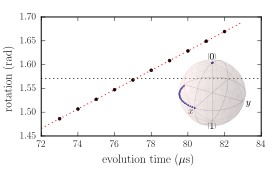
\includegraphics[width=0.85\linewidth]{../Figures/abrupt_find_tau_full.pdf} \label{FIG:get_tau}}
	\caption{(c)$d=40\, $nm}
	\label{FIG:abrupt_tau}
\end{figure}

In order to estimate the time a parity measurement would take in an experiment, we determine the parity measurement time for the abrupt and circular orbit for several data and probe qubit separations $d$ and data qubit lattice spacings $D$.

\begin{figure}[H]
	\includegraphics[width=\linewidth]{../Figures/tau_d_D}
	\caption{}
	\label{FIG:tau}
\end{figure}

The shortest parity measurement time $\tau=158\, \mu$s is achieved with the abrupt motion ($d=20\, $nm).
The parameter $d$ has the strongest influence on the parity measurement time due to the $1/r^3$ dependence of the interaction.
For a reasonable experimental implementation, we expect the parity measurement to be of the order of several milliseconds.


\section{Spin species}


\begin{table}
\begin{tabular}{ccccccccc}
	& $T_1^e$ & $T_2^{e*}$ & $T_2^e$ & $T_{2, decoupl}^e$ & $T_1^N$ & $T_2^{N*}$ & $T_2^N$ & $T_{2, decoupl.}^N$\\ \hline
P (nat. Si, SET) \cite{Pla2012}& $0.7\, $s & $55\, $ns  & $206\, \mu$s & $410\, \mu$s &  & & \\
P (puri. Si, SET) \cite{Muhonen2014}&  & $160\, \mu$s  & $1\, $ms & $560\, $ms & & $500\, \mu$s & $1.75\, $s & $35.6\, $s \\
Bi (puri. Si, CT) \cite{Wolfowicz2013} & $9\, $s &  & $2.7\, $s && && &\\
NV (puri. C, RT) \cite{Balasubramanian2009,Bar-Gill2013} & & & $1.8\, $ms & $3.3\, $ms && &&\\
NV (puri. C, $77\, $K) \cite{Bar-Gill2013} & & &  & $0.6\, $s && &&\\
SiC ($20\, $K) \cite{Christle2014} & & $1.1\, \mu$s & $1.2\, $ms & && && \\
SiC (RT) \cite{Koehl2011} & $185\, \mu$s & $214\, $ns & $40\, \mu$s &  & & && \\
\hline
\end{tabular} 
\label{lala}
\caption{\cite{Pla2012,Muhonen2014}: high field >1T low temp mK. Even good coherenc ebeing close to suurface.}
\end{table}

Donors deep in bulk show longer coherence times $T_2^e=2\, $s \cite{Tyryshkin2011} not applicable for us.

 




\section{Errors}
In this section, we will present three types of errors that we implemented in the simulation: path jitter, dephasing and data qubit displacement. The path jitter is implemented in the calculation of the Hamiltonian for each new spatial point, whereas the dephasing is introduced through a Lindblad operator. Finally, data qubit displacement is simulated by a random offset for each of the four data qubits. In connection to qubit displacement, we will also review a technique called twirling and show how it affects our simulations. Let us begin by introducing a path jitter into the simulation. 


\subsection{Benchmarking}
There are two different ways to quantify error, and we shall here quickly review them as they will be used extensively in the following sections. 

The first way to quantify error is to look at the phase $\phi$ accumulated by the probe qubit through the interaction with the data qubits. In \cite{the paper}, the phase jitter is defined as $\phi + \delta$, where $\delta$ is a small deviation from $\frac{\pi}{2}$, which is the ideal phase accumulated through one quarter of the cycle. In the paper, it was found that a phase jitter of $4.4 \%$ did not have a substantial impact on the fault-tolerance threshold. We will therefore attempt to compare the phase error in our simulation with this value whenever possible. It should be noted, however, that the data we have access to usually concerns the entire run. We will therefore compare the phase error with $2\pi$ or $\pi$. We have made the assumption that the phase error stacks, such that the phase error of $\frac{\pi}{2}$ is the same percentage as the phase error of $2\pi$ that we observe. 

The second way to quantify errors is to look at the measurement probability of correctly identifying the stabiliser state  $\ket{\psi}$, where the probability is given by $|\braket{+|\psi}|^2$ in the case of an even parity measurement and $|\braket{- |\psi}|^2$ in the case of an odd parity measurement. The need for this measure arises for example when we introduce a dephasing term in the Lindblad equation. A dephasing operator will not cause any phase error to appear since dephasing only decreases the magnitude of the Bloch vector and not its direction. Therefore, the probability of successfully identifying the stabiliser state becomes a good indicator of performance. It ranges from unity when the probe qubit state is completely pure and without phase error to 0.5 when the state has completely decohered and the measurements give entirely random outcomes. 

With these two measures in mind, let us look at the errors we introduced into the simulation and their effect on the final state. 




%\clearpage
\subsection{Path Jitter}\label{sec:jitter}
The fist error that we shall introduce is jitter present in the orbit performed by the probe qubit. The precision provided by modern MEMS control structures is about 1 nm \cite{MEMS precision} and is due to improve in the near future, but that does ont leave it impervious to noise. At first, we attempted to simulate random jumpts in the trajectory, but discontinuities in the path led to large derivative terms which in turn caused the simulation to fail. Instead, we superposed a sinusoidal motion onto the trajectory path. To add a random element, we varied the phase with which the run start while selecting the amplitude of the motion to represent the uncertainty in precision. The results can be found in Figure \ref{fig:pathjitter}, where we note that an uncertainty of about 2 nm is sufficient for staying below the phase error threshold of $4.4 \%$. Here, we are not comparing the phase jitter with the measurement probability since the probe qubit is not undergoing dephasing due to this interaction. It is sufficient to look at jitter in the $y$-direction instead of both the $x$ and $y$ direction, since the phase error is symmetric between them. 



\begin{figure}[h]
  \centering
    \includegraphics[width=0.5\textwidth]{../Figures/path_jit.pdf}
      \caption{Graph representing the percentage of phase error as a function of phase jitter in the $y$-direction (red) and in the $z$-direction (blue). There is a stronger dependence in the $z$-direction due to the $1/r^3$ term in the Hamiltonian.}
      \label{fig:pathjitter}
\end{figure}


From the graph it also becomes clear that jitter in the $z$-direction has the greatest influence. This is due to the $\frac{1}{r^3}$  term in the Hamiltonian which favours the influence of the $z$-direction. 





\subsection{Dephasing}
Next, we looked at the influence of dephasing on the measurement probabilities. In order to simulate dephasing, which is the gradual reduction of the Bloch vector in the $x$-direction, we introduced a Lindblad operator into the master equation. The operator is given by 
\beq
L  = \sqrt{\Gamma} \sigma_z,
\eeq
where $\Gamma$ is the dephasing parameter, which can also be written as $1/\tau$ where $\tau$ is the dephasing time. Since dephasing does not affect the phase accumulated over the four runs, we do not end up with a phase error, except when our state completely decoheres and the phase information becomes unavailable. Therefore, the only accurate measure of the error becomes the probability of correctly measuring the stabiliser in either the $\ket{+}$ (even parity) or $\ket{-}$ (odd parity). We ran simulations for both the abrupt and circular orbit using the $T_2$ and $T_2^*$ values in Table \ref{tab:spinspecies}. The results can be found in Figure \ref{fig:dephasing}, where each number refers to an entry in the table. 

We see that the clock transition in Bismuth does exceptionally well, but that many spin species decohere before the run is completed. This is especially notable in the case for the circular orbit, which takes approximately $10$ times longer than the abrupt orbit. It should be noted however that data for the spin species which decohere completely is for the $T_2^*$ time measured without the aid of Hahn echoes \cite{hahn} or dynamic decoupling \cite{something}. Implementing these additional techniques would significantly improve the dephasing time for many of the proposed spin species. 

As we discuss in more detail in Section \ref{sec:Outlook}, the impact of dephasing could be decreased by lowering the time needed for the probe qubit to complete one orbit around the data qubits. This would require lowering the distance $d$ between the probe qubits and the data qubits as to increase the interaction strength between them. 


\begin{figure}[H]
	\subfloat[]{\includegraphics[width=0.49\linewidth]{../Figures/abrupt-deph} \label{FIG:abr-deph}}
	\subfloat[]{\includegraphics[width=0.49\linewidth]{../Figures/circ-deph} \label{FIG:circ-deph}}
	\caption[oddeven]{The states of the probe and data qubits plotted in the Bloch sphere with a dephasing parameter of 100, which translates to a dephasing time of 10 ms. The phase of the probe qubit is not affected since no relaxation or excitation is taking place. The effect can however be seen in the probability of measuring the probe qubit in the $\ket{+}$ or $\ket{-}$ state. For complete dephasing, the probe qubit will become the maximally mixed state and the measurement outcomes are completely random. The states of the probe and data qubits plotted in the Bloch sphere with a dephasing parameter of 100, which translates to a dephasing time of 10 ms.}
	\label{FIG:deph}
\end{figure}









\begin{figure}[h]
	\centering
	\includegraphics[width=\linewidth]{../Figures/dephasing.pdf}
		\caption{A graph showing the relationship between the dephasing parameter $\Gamma$ and the probability $P(\ket{-})$ of measuring the probe qubit in the $\ket{-}$ state. In this simulation, one of the data qubits have undergone a bit-flip error. As the dephasing parameter increases, the probe qubit moves towards the maximally mixed state and the probability of measuring $\ket{-}$ goes towards 0.5.}
		\label{fig:phaseplot}
\end{figure}








\subsection{Data qubit displacement}
Yo

[BELOW LIES OLD CRAP]\\
\\

The effect of displacement of the data qubits from the ideal was investigated. Ideally the data qubits would be in a square lattice of spins precisely $D = \SI{400}{\nano\metre}$ apart, but due to inaccuracies in dopant spin placement each qubit will have small displacements from the ideal lattice position.

This is modelled by generating a uniform random displacement within a given pillbox $xy$-radius and $z$-height. Simulations from the original paper show $\textrm{radius} = \textrm{height} = \SI{6}{\nano\metre}$ to be a threshold for this scheme. The phase accumulated over 25 runs for this pillbox size is plotted as a histogram in fig.\@ \ref{fig:DisplacementPhaseHistogram}, showing a maximum phase error of $\tfrac{\pi}{4}$ for these runs. 



The effect of displacements in the $x$-$y$ plane and the $z$-axis are significantly different in magnitudes, due to the $\tfrac{1}{d^3}$ term in the Hamiltonian being most strongly affected by $z$ displacements. This effect was investigated by artificially setting displacements in these directions.

Fig.\@ \ref{fig:zoffset} shows changes in accumulated phase due to $z$-displacements. The first 2 qubits are displaced \SI{4}{\nano\metre} down, slowing the evolution and giving a noticeable phase error after half a cycle. However, qubit 4 is displaced \SI{3}{\nano\metre} upwards, reducing $d$ and resulting in faster evolution. The effect is a small phase error from the ideal $2\pi$.

Fig.\@ \ref{fig:inwarddisplacement} shows the effect of displacements in the $x$-$y$ plane. For this run, all data qubits were displaced \SI{10}{\nano\metre} inwards with respect to the circular motion. The phase error on each individual qubit is then less than that produced by the \SI{3}{\nano\metre} $z$-displacement of fig.\@ \ref{fig:zoffset}, showing the smaller sensitivity to displacement in the $x$-$y$ plane, though the overall error after all 4 qubits is greater as in the $z$-direction, +$z$ and --$z$ errors cancel out somewhat, whereas $xy$ displacement errors will always slow the evolution.

\begin{figure}[h]
	\centering
	\includegraphics[width=\textwidth]{../Figures/Displacement_phase_histogram.pdf}	
	\caption{Phase errors over 25 runs as a result of randomly generated data qubit displacements within a pillbox of half-height \SI{3}{\nano\metre} and radius \SI{6}{\nano\metre}. These values are a threshold for the proposed scheme.}
	\label{fig:DisplacementPhaseHistogram}
\end{figure}



\begin{figure}
	\centering
	\caption{Phase errors as a result of misplaced data qubits.}
	\begin{subfigure}[t]{\textwidth}
		\centering
		\includegraphics[width=0.7\textwidth]{../figures/z_offset.pdf}
		\caption{Evolution of probe qubit with data qubit displacement in the Z direction. 1st and 2nd qubits are displaced \SI{4}{\nano\metre} down, slowing the evolution, the 4th is displaced \SI{3}{\nano\metre} up with a resultant increase in phase accumulated. The overall deviation from $2\pi$ is small as a result.}
		\label{fig:zoffset}
	\end{subfigure}
	\begin{subfigure}[t]{\textwidth}
		\centering
		\includegraphics[width=0.7\textwidth]{../figures/10nm_displacement_inward.pdf}
		\caption{Phase accumulated when all 4 data qubits are displaced \SI{10}{\nano\metre} towards the centre of the circle. Other directions of \SI{10}{\nano\metre} displacements result in similar phase deviations.}
		\label{fig:inwarddisplacement}
	\end{subfigure}
	\label{fig:overall_displacement}
\end{figure}





\subsubsection{Twirling}

It is not the fact that the resultant success probabilities are lower than the even parity case that is especially concerning; this is what fault-tolerant codes are designed to cope with. Instead it is the fact that bit-flips on each qubit give a \emph{different} probability of successful detection. This means one qubit will me more prone to undetected errors than others. The fault tolerance required by the proposal assumes a symmetry between the data qubits that this breaks, making the code susceptible to logical errors.


\subsubsection{Displacement simulation}\label{sec:DisplacementSimulation}
The effect of data qubit displacement was considered in the proposal \cite{OGorman2016} using a simulation of the logical surface code operations, where the authors derived a code threshold for displacements of $R=\SI{6.1}{\nano\metre}$. We will now look more closely at the magnitude and character of errors that happen from displacements close to this threshold. 

We ran 800 simulations for even parity with no bit-flips, and 800 for odd parity with a randomly chosen bit-flip. The full dynamics of the interaction Hamiltonian derived in section \ref{sec:dipole-dipole} was simulated for each run, with randomly generated qubit displacements within the pillbox region illustrated in fig.\@ \ref{fig:pillbox} for $R = \SI{6}{\nano\metre}$, within the derived threshold. Finally, to ensure the full scheme as proposed was being implemented, randomly chosen twirling operations were added.

The 1600 simulation runs consumed 96 computer-hours, yielding the histogram in fig.\@ \ref{fig:DisplacementHistogram}. Two peaks are observed, with no significant deviation from $\pi$/$2\pi$, but the standard deviations of \num{0.265+-0.001} yield rotations from the mean of up to $\tfrac{\pi}{4}$, corresponding to a \SI{14.6}{\percent} error rate for the worst case simulated.

The standard deviation in phase represents \SI{4.2}{\percent} of $2\pi$, within the \SI{4.4}{\percent} phase jitter the proposal \cite{OGorman2016} used to derive the effect of probe jitter from the logical surface code simulation. However, projecting onto the $x$-axis to find the probability of measuring $\ket{+}\big/\ket{-}$, we find that the mean measurement success probability is \SI{98.27}{\percent} for both even and odd parity. This corresponds to a measurement error rate of \SI{1.7}{\percent}, above the code threshold of \SI{1.1}{\percent} for the surface code \cite{Wang2011,Fowler2012} despite the $R = \SI{6}{\nano\metre}$ displacement simulated being within the $R=\SI{6.1}{\nano\metre}$ threshold derived using logical simulations in the proposal \cite{OGorman2016}. 

From these simulations we conclude that the large $\tfrac{1}{r^3}$ dependence in the interaction strength has a strong enough effect on phase accumulation to bring the measurement success rate below the code threshold for the surface code. This brings into doubt the claim in the proposal \cite{OGorman2016} that the code is tolerant to physically plausible qubit displacements, and more work will be needed to resolve this and potentially calculate a new threshold.

%Thus we can conclude that, though the interaction strength has a high $\tfrac{1}{r^3}$ dependence, the parity measurement appears surprisingly tolerant to qubit displacement. Additionally, with the phase variance at the code threshold for qubit displacement being within the phase jitter parameter implemented in the proposal's logical simulations, the results of their simulation likely hold true for many likely qubit implantation techniques with precisions within the $R=\SI{6.1}{\nano\metre}$. % THIS IS BULLSHIT




\begin{figure}
	\centering
	\includegraphics[width=\columnwidth]{../Figures/Displacement_Histogram.pdf}	
	\caption{Histogram of 1600 simulation runs given random qubit displacements generated within the pillbox of fig.\@ \ref{fig:pillbox} with $R = \SI{6}{\nano\metre}$ with random twirling operations applied. The resultant measurement success probabilities \SI{98.28}{\percent} are not within the \SI{1.1}{\percent} surface code threshold \cite{Wang2011,Fowler2012}, suggesting further work may be required to characterise the code's tolerance of qubit displacements. }
	\label{fig:DisplacementHistogram}
\end{figure}


\section{Conclusions and outlook }
In this report, we have presented the results obtained from simulating the interaction between one probe qubit and four data qubits as in the proposed scheme in \cite{the paper}. 



\bibliography{papers}{}

\end{document}
